\documentclass[11pt]{article}

\usepackage[utf8]{inputenc}
\usepackage[T1]{fontenc}
\usepackage{ngerman, tikz}
\usetikzlibrary{calc, positioning}
\title{Versionsverwaltung von \LaTeX{}}
\author{Arne Brück}
\date{27.08.21}

\begin{document}
\maketitle

\section{Zusammenfassung}
Wer von Git höhrt, denkt häufig an GitHub, den Ort, der die Hälfte der
Software der Welt enthält und von dem sich die ganze Welt die Software
frei herunterladen kann.

Git ist aber unabhängig von GitHub, es ist ein Programm zur
Versionsverwaltung. Es ermöglicht auf einfache Weise Sicherheitskopien
des Projektes zu erstellen und zu späteren Zeitpunkten auf alle
früheren Veränderungen zugreifen zu können. Dies soll anhand dieses
Projektes verdeutlicht werden. Zusätzlich kann im Anschluss über
GitHub das Projekt gesichert werden oder mit anderen Menschen zusammen
komfortabel an diesem gearbeitet werden.

\section{Grundlagen}

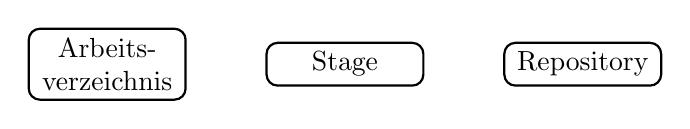
\begin{tikzpicture}
  \node (AV) [thick, draw, rounded corners, rectangle, text width = 5em, text
  centered] {Arbeits\-verzeichnis};
  \node (Stage) [thick, draw, rounded corners, rectangle, text width = 5em, text
  centered, right = of AV ] {Stage};
  \node (Rep) [thick, draw, rounded corners, rectangle, text width = 5em, text
  centered, right  = of Stage] {Repository};
\end{tikzpicture}

\end{document}

%%% Local Variables:
%%% mode: latex
%%% TeX-master: t
%%% End:
